\documentclass{standalone}

\usepackage{circuitikz}

\begin{document}

% INT_AY21_L17_Fig02_Cone_relations.png

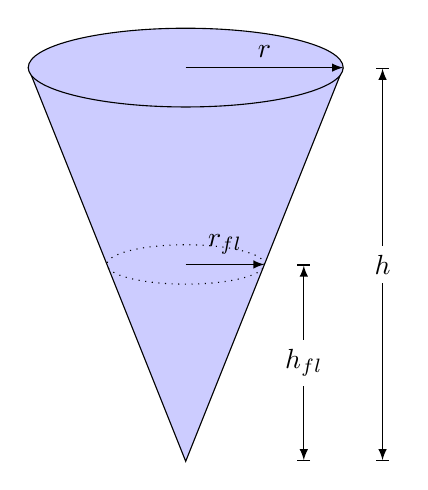
\begin{tikzpicture}[> = latex]

	% Cone bottom
	
	\filldraw [blue!20, draw = black] (2, 0) -- (0, -5) -- (-2, 0);
	
	% Cone top
	
	\filldraw [blue!20, draw = black] (0, 0) ellipse [x radius = 2 cm, y radius = 0.5 cm];
	\draw [->] (0, 0) -- node [above] {$r$} (2, 0);
	
	% Middle cross-section
	
	\draw [dotted] (0, -2.5) ellipse [x radius = 1 cm, y radius = 0.25 cm];
	\draw [->] (0, -2.5) -- node [above] {$r_{fl}$} (1, -2.5);
	
	% Height indicators
	
	\draw [|<->|] (2.5, 0) -- node [fill = white] {$h$} (2.5, -5);
	\draw [|<->|] (1.5, -2.5) -- node [fill = white] {$h_{fl}$} (1.5, -5);
	
\end{tikzpicture}

\end{document}